\section{Results}
\label{s:results}

\subsection{Exploratory Analysis}
\label{ss:eda}

In the 20{,}000-file Software Heritage sample, 52\% of files contain exactly one in-scope license detected with full confidence, 6\% a likely modified (variant) license, and 8\% several licenses; 4\% contain only out-of-scope licenses and 28\% contain no license at all (mostly \texttt{AUTHORS} files and HTML pages). Of the files with any detected license, \textbf{93.8\%} use one of our 34 licenses, which supports the chosen scope. Usage is highly skewed (Figure~\ref{fig:toplic}): MIT accounts for 70.5\% of in-scope files, followed by BSD-3-Clause (6.9\%), Apache-2.0 (6.2\%), GPL-2.0 (4.6\%), and GPL-3.0 (4.1\%), across 488 distinct license identifiers. ScanCode confidence is high (mean 99.1; 87.9\% of detections at 100). The median license file has 169 words, and 76\% of files first appeared in public history in 2015 or later. In the knowledge base, the most common conditions are include copyright (29 of 34 licenses), disclose source (14), and document changes (14); only five licenses have a network-use clause.

\begin{figure}[tb]
    \centering
    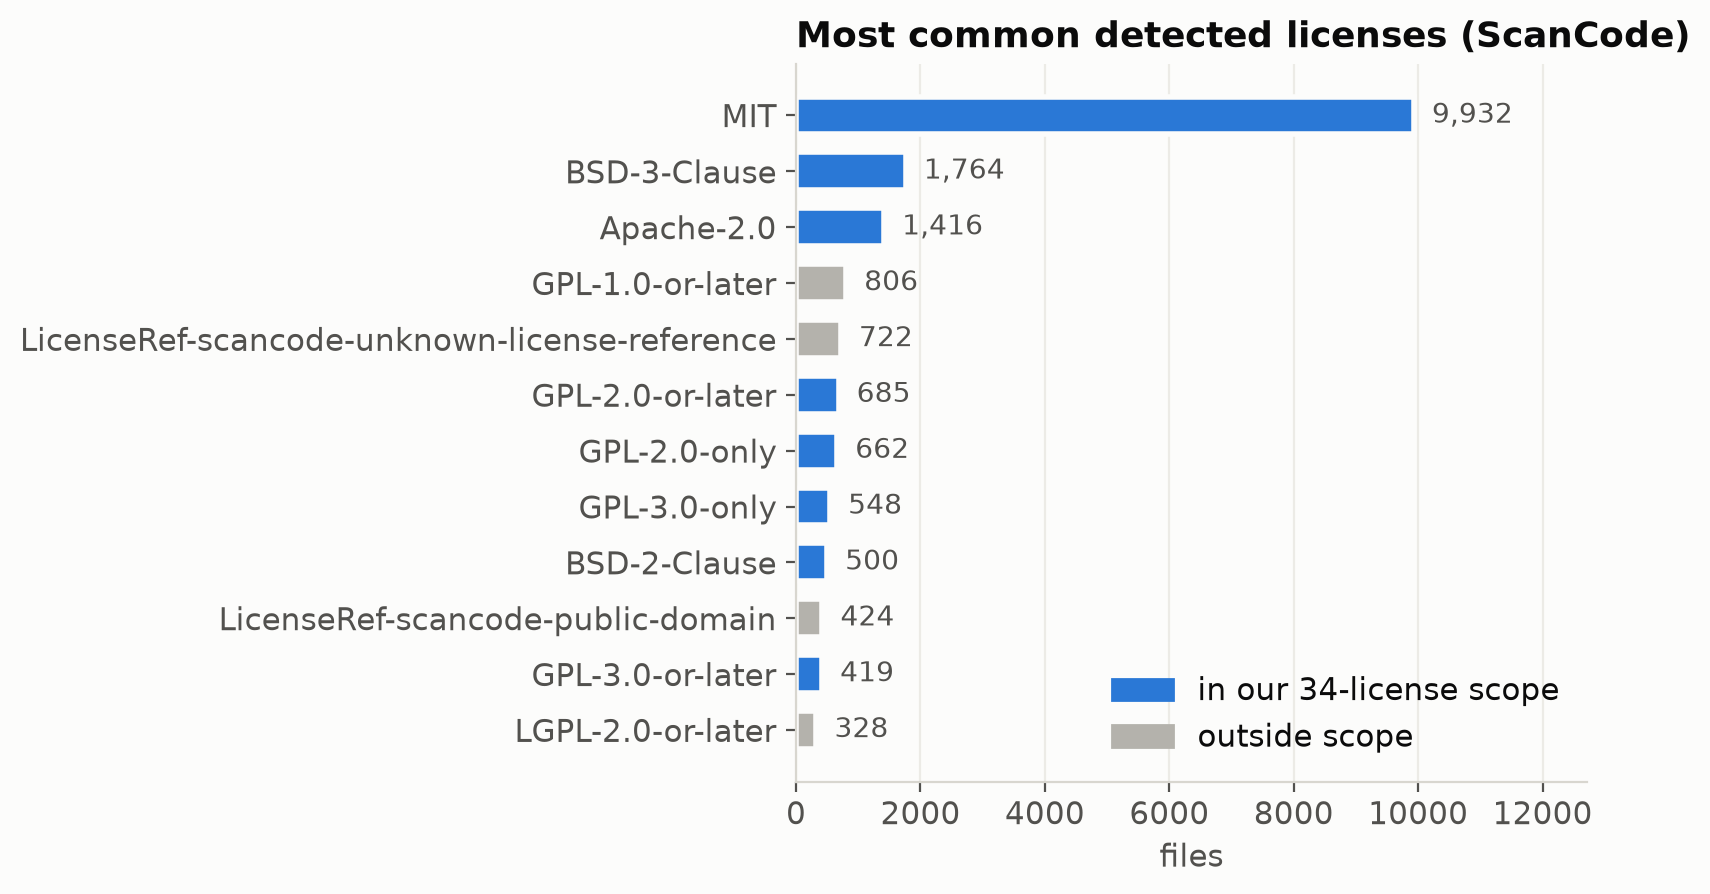
\includegraphics[width=\columnwidth]{02_top_licenses.png}
    \caption{Most common detected licenses in the Software Heritage sample (blue: in our scope).}
    \label{fig:toplic}
\end{figure}

\subsection{RQ1: Requirement-to-License Mapping}
\label{ss:rq1}

\begin{table}[tb]
    \caption{Stage 1 (gpt-oss-120b) on 104 descriptions, grouped by the number of correct licenses (answer-key size).}
    \label{tab:rq1}
    \small
    \begin{tabular}{@{}lrrrr@{}}
        \toprule
        \textbf{Correct licenses} & \textbf{n} & \textbf{Hit@1} & \textbf{Hit@3} & \textbf{Prec@3} \\
        \midrule
        1--3 (hardest) & 47 & 0.40 & 0.60 & 0.42 \\
        4--10 & 35 & 0.54 & 0.77 & 0.51 \\
        $>$10 (easiest) & 22 & 0.91 & 1.00 & 0.88 \\
        \midrule
        \textbf{All} & \textbf{104} & \textbf{0.56} & \textbf{0.74} & \textbf{0.55} \\
        \bottomrule
    \end{tabular}
\end{table}

Table~\ref{tab:rq1} and Figure~\ref{fig:rq1} summarise RQ1. Overall, the first recommendation is correct for 56\% of descriptions and a correct license appears in the top three for 74\%. Accuracy depends strongly on specificity: for broad requests (more than ten correct licenses) the model is nearly perfect (Hit@3 = 1.00), but when only one to three licenses satisfy the requirements, a correct license appears in the top three for only 60\% of descriptions and the first pick is correct for only 40\%.

Requirement violations (Figure~\ref{fig:viol}) show where recommendations go wrong. Trademark protection is the requirement most often broken (54\% of recommendations for profiles that require it), followed by ``no obligation to document changes'' (39\%), the level of copyleft (21\%), and the network-use clause (12\%); patent grant is rarely violated (4\%) and attribution never. The model also over-relies on Apache-2.0, its first choice for 30 of 104 descriptions, including cases where Apache-2.0's requirement to mark changed files violates a stated need.

\begin{figure}[tb]
    \centering
    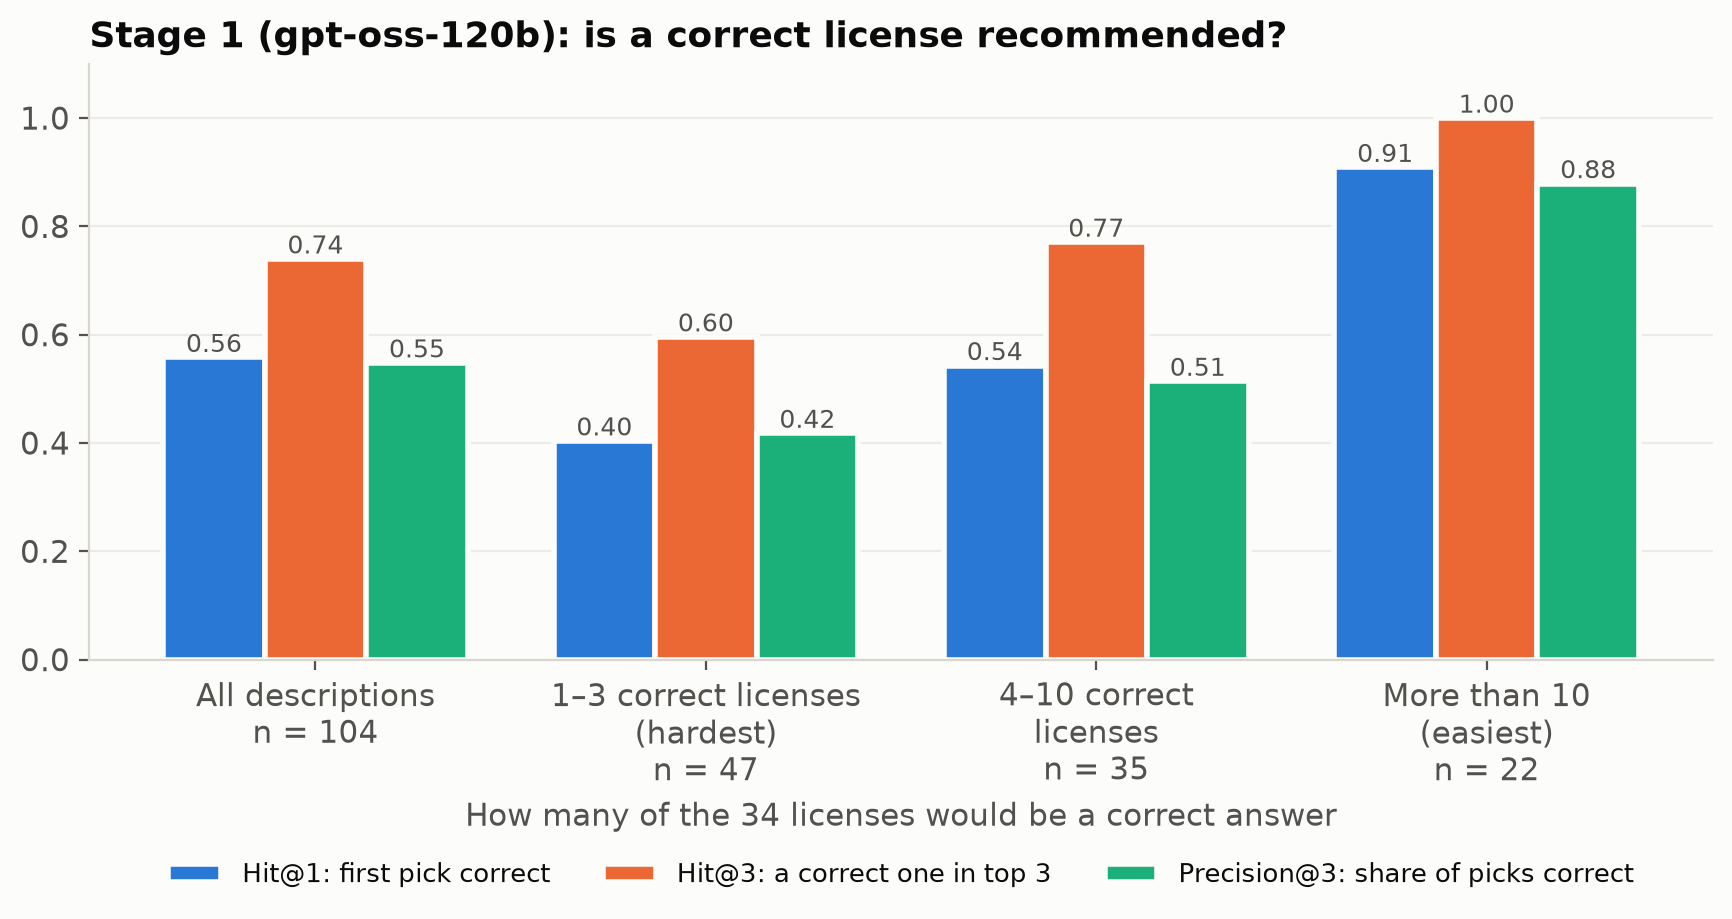
\includegraphics[width=\columnwidth]{10_stage1_hits.png}
    \caption{RQ1: Hit@1, Hit@3, and Precision@3 by answer-key size.}
    \label{fig:rq1}
\end{figure}

\begin{figure}[tb]
    \centering
    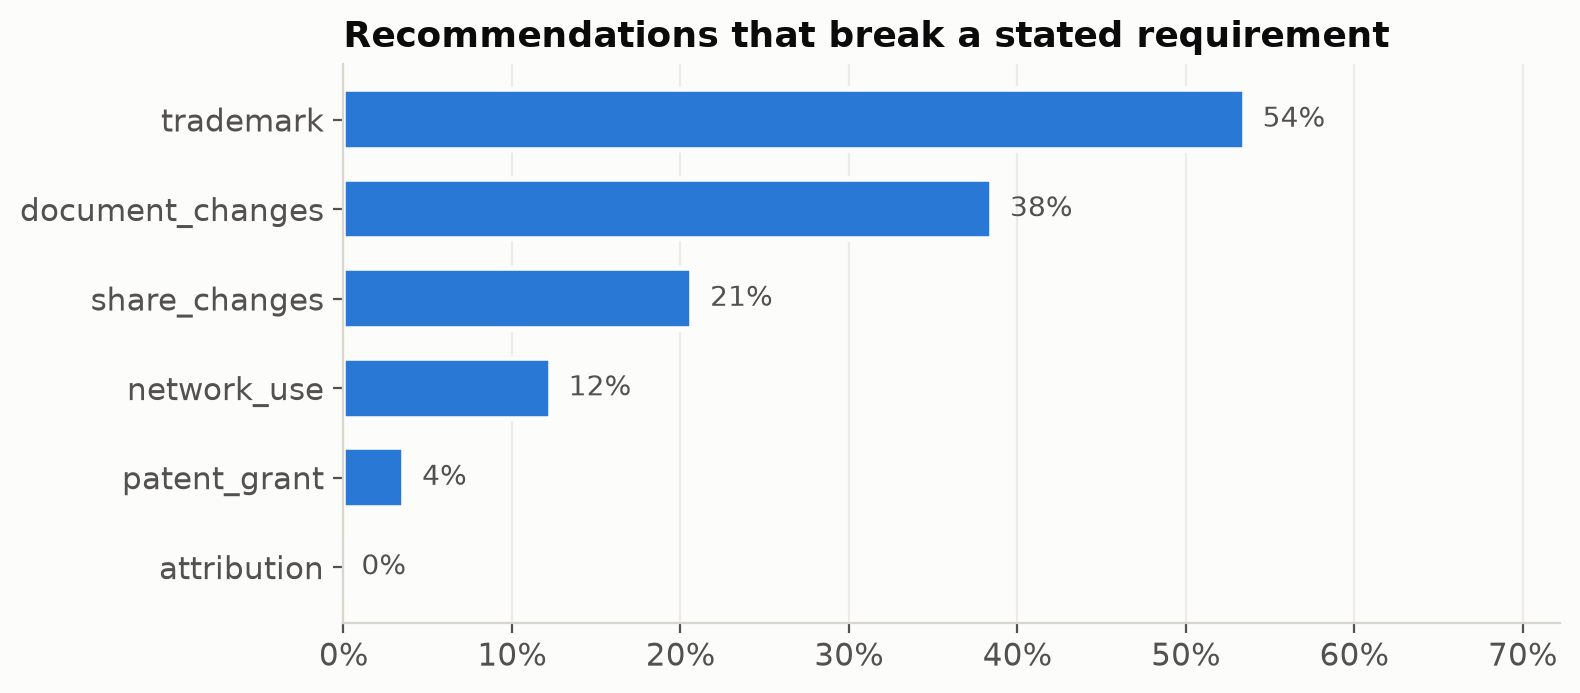
\includegraphics[width=\columnwidth]{11_stage1_violations.png}
    \caption{RQ1: share of recommendations that violate each stated requirement.}
    \label{fig:viol}
\end{figure}

\subsection{RQ2: Claim Verification}
\label{ss:rq2}

\paragraph{Label quality and agreement.} The automatic labels agree with the final human labels on 143 of 146 pairs (\textbf{97.9\%}), so the full 729-pair set can be used with confidence. On the 39 pairs labelled by both annotators, agreement is 92.3\% with Cohen's $\kappa = 0.88$, ``almost perfect'' on the Landis and Koch scale~\cite{landis1977agreement}; the second annotator could see the first label, which may inflate this value.

\begin{table}[tb]
    \caption{NLI verifiers on 146 human-labelled pairs (P/R/F1 per class).}
    \label{tab:rq2}
    \small
    \begin{tabular}{@{}llrrr@{}}
        \toprule
        \textbf{Model} & \textbf{Class} & \textbf{P} & \textbf{R} & \textbf{F1} \\
        \midrule
        \multirow{3}{*}{RoBERTa-large} & entailment & 0.900 & 0.551 & 0.684 \\
                                       & neutral & 0.583 & 0.745 & 0.654 \\
                                       & contradiction & 0.804 & 0.900 & 0.849 \\
        \multicolumn{2}{@{}l}{\quad accuracy 0.733; macro-F1 0.729} & & & \\
        \midrule
        \multirow{3}{*}{DeBERTa-v3-large} & entailment & \textbf{0.944} & \textbf{0.694} & \textbf{0.800} \\
                                          & neutral & 0.672 & 0.872 & 0.759 \\
                                          & contradiction & 0.898 & 0.880 & 0.889 \\
        \multicolumn{2}{@{}l}{\quad accuracy \textbf{0.815}; macro-F1 \textbf{0.816}} & & & \\
        \bottomrule
    \end{tabular}
\end{table}

\paragraph{Model comparison.} Table~\ref{tab:rq2} reports both verifiers on the human-labelled pairs. DeBERTa-v3-large outperforms RoBERTa-large-MNLI on every class, with accuracy 0.815 versus 0.733 and macro-F1 0.816 versus 0.729. On all 729 automatically labelled pairs the ranking is the same (accuracy 0.809 versus 0.782). We therefore use DeBERTa as the verifier.

\begin{table}[tb]
    \caption{DeBERTa confusion matrix on 146 human-labelled pairs (rows: human label; columns: prediction).}
    \label{tab:cm}
    \small
    \begin{tabular}{@{}lrrr@{}}
        \toprule
        & \textbf{entail.} & \textbf{neutral} & \textbf{contrad.} \\
        \midrule
        entailment & \textbf{34} & 14 & 1 \\
        neutral & 2 & \textbf{41} & 4 \\
        contradiction & 0 & 6 & \textbf{44} \\
        \bottomrule
    \end{tabular}
\end{table}

\paragraph{Error profile.} The confusion matrix (Table~\ref{tab:cm}) shows that the verifier errs on the side of caution. When it predicts entailment (shown to users as \emph{verified}) it is correct 94\% of the time, and it never labelled a false (contradicted) claim as entailed. Its main weakness is recall on true claims: 14 of 49 entailed claims (29\%) were judged neutral and would appear as \emph{unverified}. Six contradictions were also judged neutral, and four neutral claims were wrongly flagged as contradictions. Figure~\ref{fig:recall} breaks entailment recall down by label: claims about document changes (91\%), liability (90\%), and distribution (84\%) are usually confirmed, whereas claims about commercial use (21\%), same-license copyleft (25\%), and network use (25\%) rarely are. These are the labels for which a license states the obligation in different terms from the claim; for example, a license says ``sell'' or ``charge a fee'' rather than ``commercial use''.

\begin{figure}[tb]
    \centering
    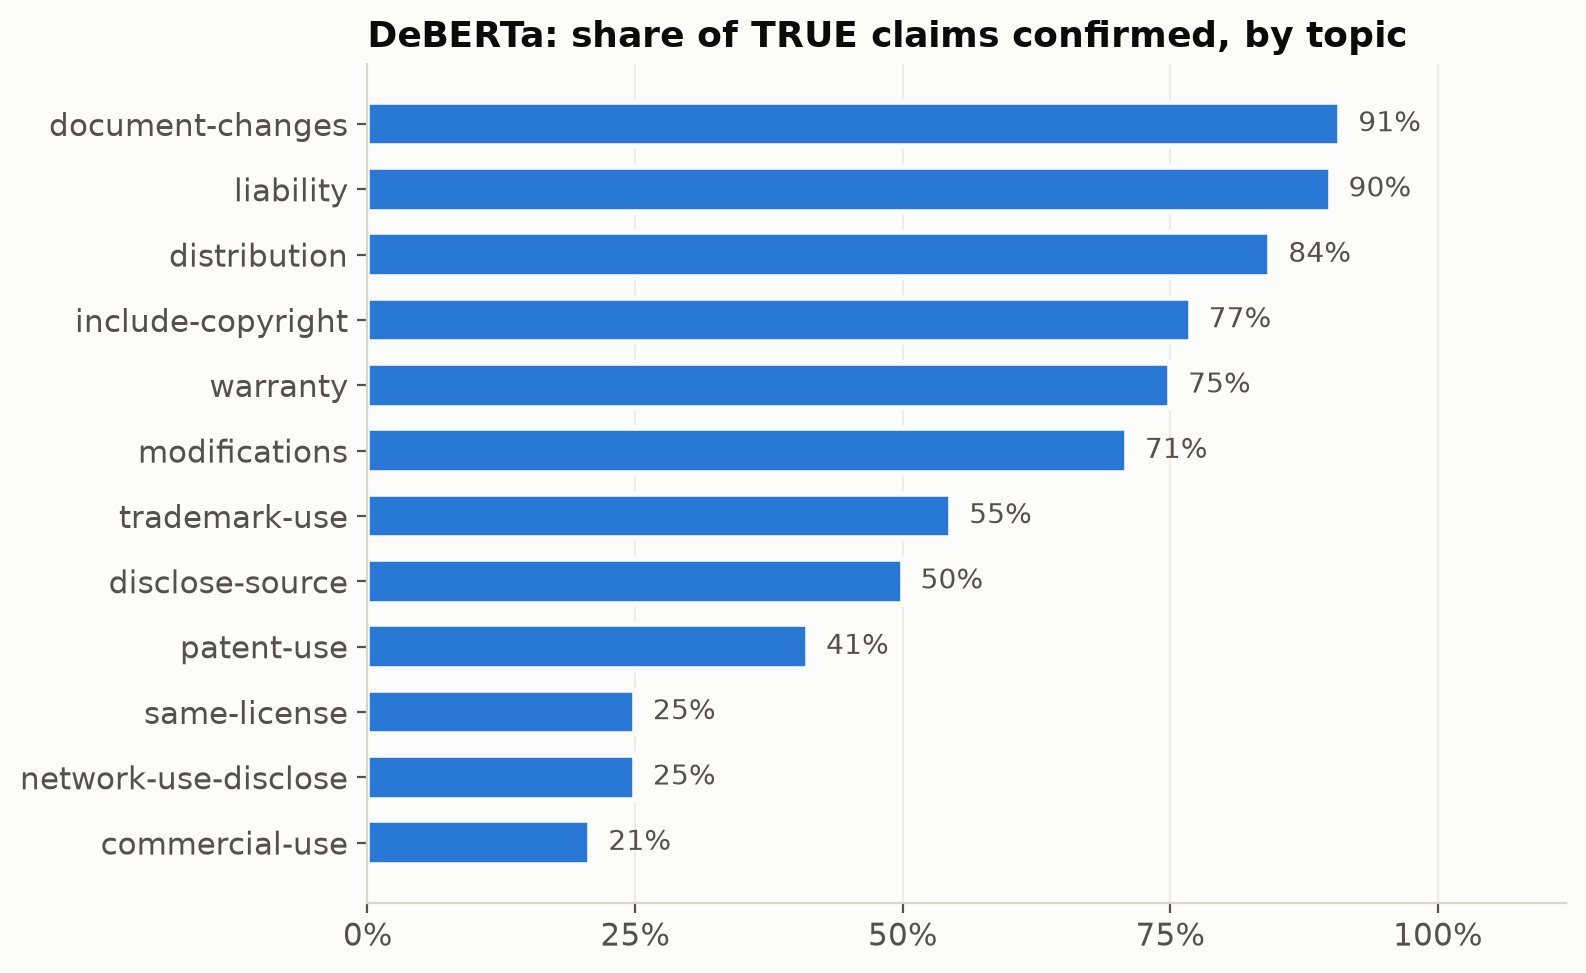
\includegraphics[width=\columnwidth]{09_nli_recall_by_label.png}
    \caption{RQ2: share of true claims confirmed by DeBERTa, by license label (729 automatically labelled pairs).}
    \label{fig:recall}
\end{figure}

\subsection{RQ3: Explanation Faithfulness (Preliminary)}
\label{ss:rq3}

Two complete pipeline runs produced 19 claims across six license recommendations. All 19 quotes (100\%) were found verbatim in their cited clauses, indicating that clause-level grounding constrains the explainer's quotations. Of the claims, 11 (58\%) were verified, 7 (37\%) unverified, and 1 (5\%) contradicted. Manual inspection of the unverified claims shows that most were correct statements of copyleft or commercial-use terms, consistent with the RQ2 error profile, and the single contradicted claim (an accurate paraphrase of AGPL-3.0 section~6) was a verifier false positive. A systematic comparison with an unverified baseline is left to Phase~2.
